\subsection{Принцип работы}

На данном микроконтролере существует 6 различных портов:
\begin{itemize}
    \item GPIOA
    \item GPIOB
    \item GPIOC
    \item GPIOD
    \item GPIOE
    \item GPIOF
\end{itemize}   


\begin{figure}[h!]
		\centering
		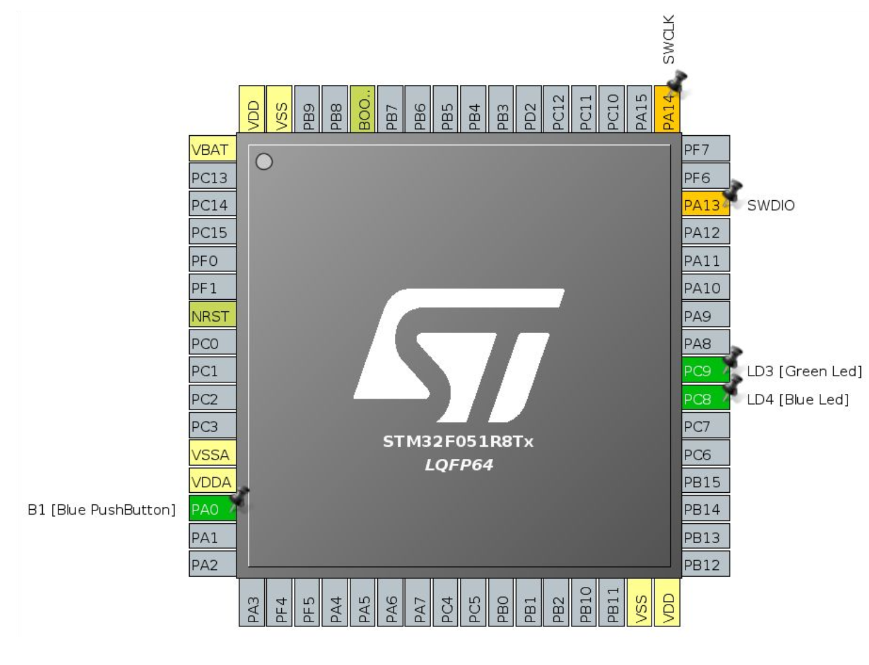
\includegraphics[width=1\linewidth]{pics/scheme.png}
		\caption{Порты и пины}
		\label{drebezg}
\end{figure}

У каждого порта по 16 пинов. Однако в большинстве случаев в виду органиченности ножек микроконтролера не все порты реализуются полностью. В случае нашей платы: три пина заняты под два стедиода и одну кнопку, два пина заняты для соединения с программатором. 


Управление с пинами осуществляем с помощью LL-функций.

\begin{verbatim}
    //обычная функция для записи в регистр
    LL_GPIO_SetPinMode(GPIOx, LL_GPIO_PIN_x, Regime) ;
    //За один раз данная функция фонкфигурирует только один пин.

    //Настройка типа цифрового выхода
    LL_GPIO_SetPinOutputMode(GPIOx, LL_GPIO_PIN_x, Regime);
    // 1) Regime = LL_GPIO_OUTPUT_PUSHPULL
    // 2) Regime = LL_GPIO_OUTPUT_OPENDRAIN
    // Аналогично только один пин.
    
    //Функции для изменения выходного состояния
    LL_GPIO_WriteOutputPort(GPIOx, output_value); -> ODR
    
    LL_GPIO_WriteOutputPin(GPIOx, bits_of_pins); -> BSRR
    
    LL_GPIO_ResetOutputPin(GPIOx, bits_of_pins); -> BRR
    //Можно писать в несколько пинов!

\end{verbatim}


\subsection{Дребезг контактов}


\begin{figure}[h!]
		\centering
		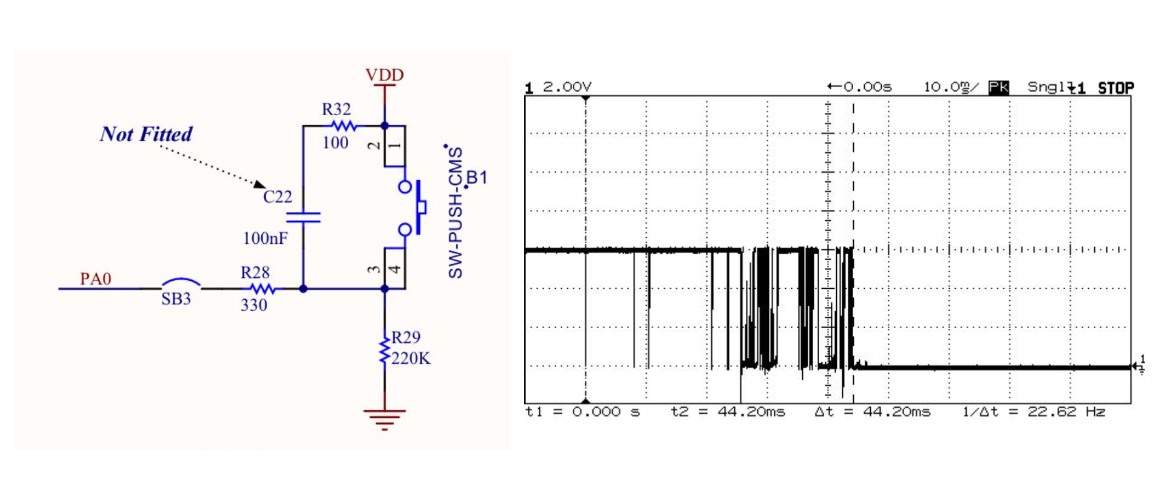
\includegraphics[width=1\linewidth]{pics/drebezg.png}
		\caption{Устройства подключения кнопки и график с дребезгом}
		\label{drebezg}
\end{figure}

На рис.\ref{drebezg} показано подключение кнопки $USER$ на нашей отладочной плате.
Синяя кнопка заземлена, так же подключена в пину $PA0$. 
	
	
Проблема дребезга заключается в том, что при нажатии на кнопку происходит на самом деле не только лишь одно нажатие, а еще и большое количество ложных переключений, которые приводят к ложным положительным срабатываниям. Наивным образом график этого процесса в реальном и в идеальном случаях показан на рис. \ref{drebezg} и рис.\ref{ideal_graph}.

Методы борьбы с дребезгом.

\textbf{Аналоговый}:

Установка низкочастотный фильтр для фильтрации дребезга, который мы предсавляем как высокочастотный сигнал.

\textbf{Программные методы}:

Создание некоторой задержки, после которой мы снова опрашиваем кнопку, чтобы удостовериться, что кнопка действительно была нажата.


В нашей работе мы пытались бооться с дребезгом различными программными методами: наинвым образом, а так же более совершенным. Ниже приводим код наивной и более совершенной реализации:


    Наивная реализация.
\begin{verbatim}
    // 1 - кнопка нажата; 0 - отжата
    // Проверяем состояние регистра
    status = LL_GPIO_IsInputPinSet(GPIOA, LL_GPIO_PIN_0); 
    
    if (status == 1) 
    {   
        is_on = 1;
        delay_0.1ms();
        
        if (is on)
            LL_GPIO_ResetOutputPin(GPIOC, LL_GPIO_PIN_8) 
        else 
            LL_GPIO_SetOutputPin(GPIOC, LL_GPIO_PIN_8);
    }
\end{verbatim}
    
Более совершенная реализация
\begin{verbatim}
    
    // Проверяем состояние регистра
    status = LL_GPIO_IsInputPinSet(GPIOA, LL_GPIO_PIN_0);
 
    if (status)
    {
      counter++;     // Устанавливаем счетчик
      delay_10ms();
    }
        
    if (counter >= 5)                                   
    {
      LL_GPIO_ResetOutputPin(GPIOC, LL_GPIO_PIN_8);
        
       while(1)
        Show();     // Функция для вывода чего-нибудь
     }
   
    else
      LL_GPIO_SetOutputPin(GPIOC, LL_GPIO_PIN_8);
\end{verbatim}



\begin{figure}[h!]
		\centering
		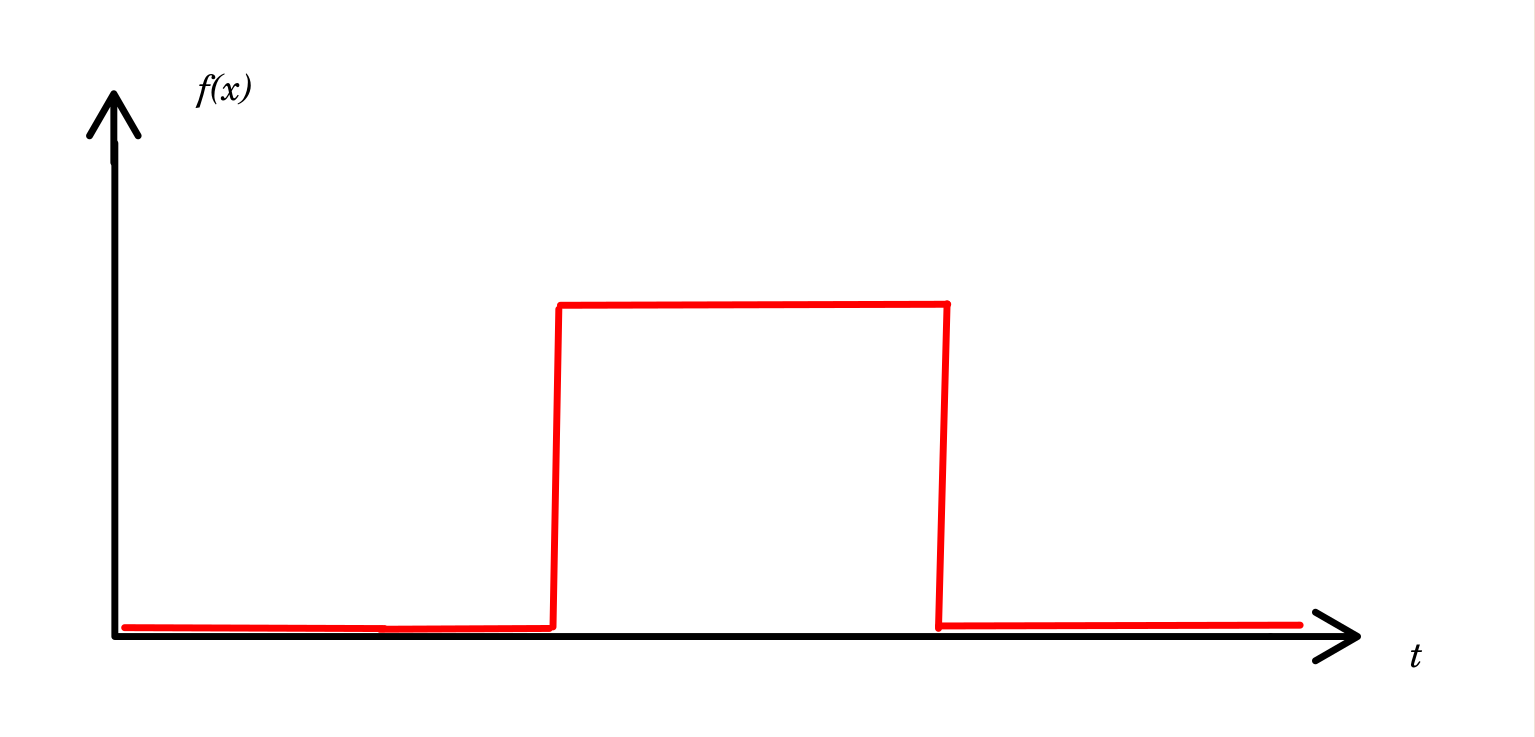
\includegraphics[width=1\linewidth]{pics/ideal_sing.png}
		\caption{Идеальный график сигнала}
		\label{ideal_graph}
\end{figure}
